\documentclass[11pt,a4paper]{article}

\usepackage{epsfig}
\usepackage{multicol}

\usepackage[utf8]{inputenc}
\usepackage[brazil]{babel}
\usepackage{fancyheadings}
\usepackage{amsmath}
\usepackage{calrsfs}
\usepackage{enumerate}
\usepackage{enumitem}   
\DeclareGraphicsExtensions{.png,.pdf}
\usepackage{amsmath, amsfonts, amssymb}
\usepackage{esint}
\usepackage{graphicx}
\usepackage{multicol}
\usepackage{tasks}
\usepackage[utf8]{inputenc}
\usepackage{mathrsfs} % Transformada de Laplace
\usepackage{indentfirst}
\usepackage{xcolor}

% As margens
\setlength{\textheight}{24.0cm}
\setlength{\textwidth}{17.5cm}
\setlength{\oddsidemargin}{2.0cm} % Margens reais desejadas
\setlength{\evensidemargin}{2.0cm} % 2+17.5+1.5=21cm (largura A4)
\setlength{\topmargin}{1.5cm} % 1.5+1.6+1.0+24.0+1.6=29.7cm
\setlength{\headheight}{1.6cm} % (altura A4)
\setlength{\headsep}{1.0cm}
\setlength{\columnsep}{1.5cm} % Coluna = 8cm ((17.5-1.5)/2)
\addtolength{\oddsidemargin}{-1in}
\addtolength{\evensidemargin}{-1in}
\addtolength{\topmargin}{-1in}
\setlength{\footskip}{0.0cm}


% Novos comandos
\newcommand{\limite}{\displaystyle\lim}
\newcommand{\integral}{\displaystyle\int}
\newcommand{\somatorio}{\displaystyle\sum}
\newcommand{\mat}[1]{\mbox{\boldmath{$#1$}}} 

\pagestyle{fancy}


\usepackage{lipsum}

\lhead{

\includegraphics[width=1cm]{brasao.png}
}

\rhead{ 
\sc\textbf{U}niversidade \textbf{F}ederal do \textbf{C}eará\\
Campus Quixadá\\ Lista 4 de Eletromagnetismo}

\cfoot{}

\begin{document}

	\begin{center}
		\Large Eletrostática - Potencial Elétrico e Condições de Contorno. 
	\end{center}

\begin{flushleft}
\textbf{Nome:} Mateus Sousa Araújo. \\
\textbf{Matrícula:} 374858. \\
\textbf{Professor:} Antônio Joel Ramiro de Castro. \\
\textbf{Curso:} Engenharia de Computação. \\
\end{flushleft}

\begin{enumerate}

\item \textbf{Griffiths - Cap. 3 - Problema 3.14.}

Um tubo retangular que corre paralelo ao eixo $z$ (de $-\infty$ a $+\infty$), tem três lados de metal aterrados, em $y = 0$, $y = a$ e $x = 0$. O quarto lado, em $x = b$, é mantido em um potencial específico $V_0(y)$.

\begin{enumerate}
\item Desenvolva uma fórmula geral para o potencial no interior do tubo.
\item Encontre o potencial explicitamente, para o caso $V_0(y) = V_0$ (uma constante).
\end{enumerate}


\textbf{RESOLUÇÃO}

\begin{enumerate}

\item 

\begin{figure}[h]	
\centering % para centralizarmos a figura	
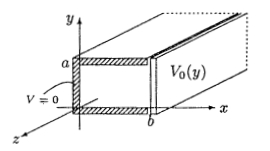
\includegraphics[width=6cm]{Selection_084.jpg} 
\end{figure}

Com a figura acima, temos as seguintes condições de contorno:

\begin{enumerate}
\item $V(x,0) = 0$
\item $V(x,a) = 0$
\item $V(0,y) = 0$
\item $V(b,y) = V_0(y)$
\end{enumerate}

Precisamos resolver a equação de Laplace para esse caso:

$$\displaystyle\dfrac{\partial ^2 V}{\partial x^2} + \displaystyle\dfrac{\partial ^2 V}{\partial y^2} = 0$$

Podemos considerar duas funções em $x$ e $y$ que compõem o potencial. 

$$V(x,y) = \varphi (x) \psi (y)$$

Fazendo as derivadas segundas de cada função de acordo com a equação de Laplace, temos:

$$V_{xx} = \psi (y) \varphi '' (x) $$
$$V_{yy} = \varphi (x) \psi '' (y) $$ 

Somando na equação de Laplace e dividindo ambos temos por $1/V$, obtemos:

$$\displaystyle\dfrac{1}{V}(\psi (y) \varphi '' (x) + \varphi (x) \psi '' (y)) = 0$$

$$\displaystyle\dfrac{1}{\varphi (x)}\varphi'' (x) + \displaystyle\dfrac{1}{\psi (y)}\psi'' (y) = 0$$

$$f(x) + g(y) = 0$$

Podemos chamar $f(x)$ de uma constante $c_1$ e $g(y)$ de outra constante $c_2$. Dessa forma:

$$c_1 + c_2 = 0$$
$$c_1 = -c_2$$
$$c_1 = k^2$$

Temos duas equações de 1 ordem:

\begin{equation}
\displaystyle\dfrac{1}{\varphi (x)}\varphi'' (x) = c_1
\label{eq1}
\end{equation}

\begin{equation}
\displaystyle\dfrac{1}{\psi (y)}\psi'' (y) = c_2
\label{eq2}
\end{equation}

Em $\ref{eq1}$ temos:

$$\displaystyle\dfrac{\partial ^2 \varphi}{\partial x^2} = k^2\varphi$$

Para esse caso, temos uma solução da seguinte forma:

\begin{equation}
\varphi (x) = A e^{kx} + B e^{-kx}
\label{eq3}
\end{equation}

Em $\ref{eq2}$ temos:

$$\displaystyle\dfrac{\partial ^2 \psi}{\partial y^2} = - k^2\psi$$

Para esse caso, temos uma solução da seguinte forma:

\begin{equation}
\psi (y) = C \sin(ky) + D \cos(ky)
\label{eq4}
\end{equation}

Aplicando a 3ª condição em $\ref{eq3}$, temos:

$$V(0,y) = \varphi (0) \psi (y) = 0$$

Da condição acima, temos que $\varphi (0) = 0$. Aplicando esse resultado em $\ref{eq3}$, temos:

$$B = -A$$

Aplicando a 1ª condição em $\ref{eq4}$, temos:

$$V(0,y) = \varphi (x) \psi (0) = 0$$ 

Da condição acima, temos que $\psi (0) = 0$. Aplicando esse resultado em $\ref{eq4}$, temos:

$$D = 0$$

Aplicando a 2ª condição em $\ref{eq4}$, temos:

$$V(0,y) = \varphi (x) \psi (a) = 0$$ 

Da condição acima, temos que $\psi (a) = 0$. Substituindo esse valor em $\ref{eq4}$, temos que:

$$ka = n\pi$$ 

$$k = \displaystyle\dfrac{n\pi}{a}$$ 

onde, $n = 0, 1, 2, 3, ...$

Retornando para $V(x,y)$, temos:

$$V(x,y) = (A e^{kx} + B e^{-kx}) (C \sin(ky) + D \cos(ky))$$

$$V(x,y) = (2AC)(e^{n\pi x/a} - e^{-n\pi x/a}) \sin\left(\displaystyle\dfrac{n\pi y}{a}\right)$$

$$V(x,y) = (2AC)\sinh\left(\displaystyle\dfrac{n\pi x}{a}\right) \sin\left(\displaystyle\dfrac{n\pi y}{a}\right)$$

Já que $2AC$ é uma constante arbitrária, temos:

\begin{equation}
V(x,y) = \displaystyle\sum_{n=1}^\infty C_n \sinh\left(\displaystyle\dfrac{n\pi x}{a}\right) \sin\left(\displaystyle\dfrac{n\pi y}{a}\right) 
\label{eq5}
\end{equation}

Aplicando a última condição em $\ref{eq5}$, temos:

$$\displaystyle\sum C_n \sinh\left(\displaystyle\dfrac{n\pi b}{a}\right) \sin\left(\displaystyle\dfrac{n\pi y}{a}\right) = V_0(y)$$

Por definição, temos:

$$C_n \sinh\left(\displaystyle\dfrac{n\pi b}{a}\right) = \displaystyle\dfrac{2}{a}\displaystyle\int_0^{a} V_0(y) \sin\left(\displaystyle\dfrac{n\pi y}{a}\right) \ dy$$

Portanto, chegamos:

$$C_n = \displaystyle\dfrac{2}{a\sinh(n\pi b/a)}\displaystyle\int_0^{a} V_0(y) \sin\left(\displaystyle\dfrac{n\pi y}{a}\right) \ dy$$

\item

$$C_n = \displaystyle\dfrac{2}{a\sinh(n\pi b/a)}V_0\displaystyle\int_0^{a} \sin\left(\displaystyle\dfrac{n\pi y}{a}\right) \ dy$$

No entanto, temos:

$$\int_0^{a} \sin\left(\displaystyle\dfrac{n\pi y}{a}\right) \ dy = 
		\begin{cases}
			0,\, \textrm{se n for par} \\
			\displaystyle\dfrac{2a}{n\pi},\, \textrm{se n for ímpar} \\
		\end{cases}
	$$
	
Com as condições acima, podemos concluir:

$$V(x,y) = \displaystyle\dfrac{4V_0}{\pi}\displaystyle\sum_{n=1,3,5,...}\displaystyle\dfrac{\sinh(n\pi x/a) \sin(n\pi y/a)}{n \sinh(n\pi b/a)}$$

\end{enumerate}


\item \textbf{Griffiths - Cap. 3 - Problema 3.19.}

Suponha que o potencial $V_0(\theta)$ na superfície de uma esfera é especificado e que não há carga dentro ou fora da esfera. Mostre que a densidade de carga na esfera é dada por

$$\sigma (\theta) = \displaystyle\dfrac{\epsilon_0}{2R} \displaystyle\sum_{l=0}^\infty (2l + 1)^2 C_l P_l (\cos \theta)$$

onde 

$$C_l = \displaystyle\int_0^\pi V_0(\theta) P_l (\cos \theta) \sin \theta \ d\theta.$$

\textbf{RESOLUÇÃO}

Podemos usar a seguinte relação:

$$\sigma (\theta) = \epsilon_0 \displaystyle\sum_{l=0}^\infty (2l + 1) A_l R^{l-1} P_l (\cos \theta)$$

Temos que:

$$A_l = \displaystyle\dfrac{2l + 1}{2R^l} \displaystyle\int_0^\pi V_0(\theta) P_l (\cos \theta) \sin \theta \ d\theta$$

Juntando as duas, temos:

$$\sigma (\theta) = \epsilon_0 \displaystyle\sum_{l=0}^\infty (2l + 1)^2 C_l P_l (\cos \theta)$$

O valor para $C_l$, fica:

$$C_l = \displaystyle\int_0^\pi V_0(\theta) P_l (\cos \theta) \sin \theta \ d\theta.$$


\item \textbf{Griffiths - Cap.3 - Problema 3.27.}

Quatro partículas (uma de carga $q$, uma de carga $3q$ e duas de carga $-2q$) estão dispostas como mostra a figura abaixo, cada uma delas a uma distância $a$ da origem. Encontre uma fórmula simples aproximada para o potencial, válida em pontos distantes da origem. (Expresse sua resposta em coordenadas esféricas.)

\begin{figure}[h]	
\centering % para centralizarmos a figura	
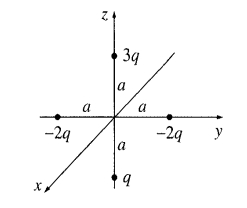
\includegraphics[width=5cm]{Selection_085.jpg} 
\end{figure}

\textbf{RESOLUÇÃO}

$$p = (3qa - qa)\hat{\mat{z}} + (-2qa - 2q(-a))\hat{\mat{y}} = 2qa \hat{\mat{z}}$$

Para a fórmula do potencial, temos:

$$V = \displaystyle\dfrac{1}{4\pi \epsilon_0} \displaystyle\dfrac{p \cdot \hat{\mat{r}}}{r^2}$$

Temos também que:

$$p \cdot \hat{\mat{r}} = 2qa\hat{\mat{z}} \cdot \hat{\mat{r}} = 2qa \cos \theta$$

Dessa forma, concluímos que o dipolo fica:

$$V = \displaystyle\dfrac{1}{4\pi \epsilon_0} \displaystyle\dfrac{2qa \cos \theta}{r^2}$$



\end{enumerate}
	
\end{document}